% -*- mode: latex; mode: auto-fill; coding: utf-8; -*-

\chapter{Sky}
The sky is an essential part of an outdoor environment, whether it is
night, day, cloudy or clear sky plays an important role in setting the
mood of the scene. 
%Each of these different looking skies are composed
%of different phenomena that needs to be modeled and simulated by
%differently.
The sky is an ever changing part of an outdoor scene
and depends on many parameters including both the time of the day and
on the weather conditions.
%
This makes it a hard effect to simulate and visualize, but because it
is such a central part of an outdoor setting, it must be included in
the rendering.
%
One possibility is to simulate all important real world conponents
influencing the apperance of the sky. This could e.g involved complex
weather forecast models or other large models, but because there are
so many complex phenomena influencing it apperance this cannot be done
in real time. Instead we have chosen the most obvious effects and
tried to create believable visualizations of those.

When rendering a scene it is important that the overall LOD
matches, to convince the user of our illusion. This means that if we
have a scene with high detailed objects, we also need to render the
sky in high detail. If we had a simple scene, then it could be enough to
simulate the sky by a simple light blue background color. This
approach works fine when used e.g. together with cartoon shading. But
as objects in the scene becomes more detailed and realistic looking
this simple approach makes the sky stand out. 
%
Simulating a more realistic looking sky can and have been done many
different way. Some developers use what is known as \emph{sky boxes}
\citebook{page~338-339}{RTR2},
which is a technique that maps images of the sky onto a box. This box
then surrounds the entire scene where the camera is inside the box at
all times, making the illusion of fare stretching planes by using
simple images.
%
One problem with using a box when doing this, is that the edges
between the images on different sides of the box are apparent as
artifacts when looking directly at them. To get around this problem,
developers instead use a sphere or dome as the basic geometry, and
hence the name sky dome, when rendering the sky. The main difference
between these two approaches is the texture mapping of the
images. When mapping images onto a box a straight forward approach can
be used, but when using a dome this step becomes much more tricky.
%
Although this approach can give fine results, the sky remains frozen
in time, which makes it unrealistic when looking at it fore longer
periods in time. 
%
So we have take up the challenge of simulating the image animation on
a sky dome.

\section{Sky domes}
We have chosen to using two sky spheres, one inner sphere for
rendering white clouds with alpha transparency, and an outer sphere to
render a background color which can change based on the time of day.
We also include cloud animation based on a simple wind model, so
the clouds change over time.

\subsection{Geometry}
We have tried two different ways on generating the sphere
geometry. The first method used was the traditional longitudinal/latitude
sphere commonly used for geographical maps. This
however gave very obvious image stretching artifact at the poles
because of oversampling in these regions. Instead we now use geodesic
spheres which consist of equilateral triangles that are beautifully
constructed by recursively subdivision of an icosahedron until the
required LOD is attained.

\subsection{Sun}

\subsection{Atmospheric dome}
What phenomena drives the coloring of the sky, making it so beautiful
with it shades of blue and red?
This is the questing ask by researchers studying 
\emph{atmospheric scattering}. This subject has been studied in great detail
and lots of complex theories and models has been developed within the field.
We however have chosen not dig deep into this subject because it could
be an entire subject of its own.
%
However, to color our sky we use a simple model based on color
gradients as described in \citeabook{abad2006}.
Where the atmospheric dome is colored based on time, height, and the
location of the sun.

\begin{figure}[!h]
  \centering
  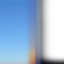
\includegraphics[width=5cm]{EarthClearSky2}
  \caption{Color gradient used to color the atmospheric dome. The
    white on the right is alpha transparency.}
  \label{fig:sky-gradient}
\end{figure}

We use the color gradient in figure
\ref{fig:sky-gradient}, borrowed from the Caelum
framework\footnote{\url{http://www.ogre3d.org/tikiwiki/Caelum}}.
using the height for texture mapping in the y direction and time of
day in the x direction. This divides time into four periods: day,
night, sunrise and sunset by first going positive along the x direction,
and then the other way.
One possible extension here is to include the location or angle of the
sun to make a more beautiful sunrise and sunset.

The alpha channel seen on the right in figure \ref{fig:sky-gradient}
is used at night to enable rendering of stars. We render stars simple
by pregenerating a black square image with randomly placed pixels,
painted shades of white, in a circle round the center of the
image. This images is then alpha blended with the color gradient based
on normalized x and z coordinates of the atmospheric dome.

\subsection{Cloud Dome}

\subsubsection{Cloud texture}
We have chosen to use a procedural generated image to visualize the
clouds. By take this approach we can change their appearance and
generate very different looking clouds by only altering a few
parameters that is supplied to the generation algorithm.
%
We have furthermore chosen a three dimensional image because this
eases texture mapping when the image is to be mapped onto the sphere.
%
To generate the cloud image we have been inspired by an Internet
homepage\footnote{\url{http://freespace.virgin.net/hugo.elias/models/m_clouds.htm}
  \\Be warned though, this homepage does not use Perlin noise as they
  say but value lattice noise.}
describing how to use procedural generation and
image layering/composition in combination to produce texture that
looks like real clouds.
Because this is a large subject we have dedicated another chapther for
it describtion. Here it is enought to say that we generate a three
dimensional texture which is ensured to be wrapable along all three
dimensions.

\subsubsection{Texture mapping - animation}
The basic texture mapping scheme, is to put the three dimensional
texture into a unit cube, and use texture coordinates based on the
unit sphere to make a direct mapping which avoids texture stretching.

If we only did this, the a large portion of the generated texture
would not be used.

So besides the basic texture mapping scheme, we have introduced
texture coordinate animation. This has been done by modeling the wind.

\subsubsection{Wind simulation}
We have implemented a simple wind simulation algorithm which is
inspired by Brownian motions. It works by having a current and future
wind direction. The future direction is generated randomly based on
the current and are normal distributed. Switching from the current and
future direction is done by interpolating the two, and switching 






%%% Local Variables:
%%% mode: latex
%%% TeX-master: t
%%% TeX-PDF-mode: t
%%% End:

